% Chapter Template

\chapter{Building a quantum processor} % Main chapter title

\label{Chapter4} % Change X to a consecutive number; for referencing this chapter elsewhere, use \ref{ChapterX}

\HRule
\vspace{0.5cm} \hspace{2cm}
\small
\hangindent=4cm
\\
        ``\emph{Scalability is the future}"
\\ \\
\hangindent=4cm
\begin{flushright}
--? \\
\end{flushright}

\vspace{0.5cm}

\noindent \HRule
\clearpage

\begin{figure*}
	\centering
	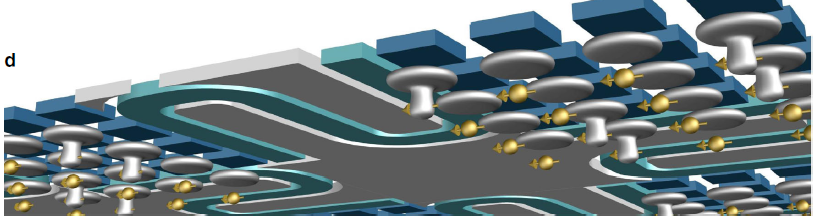
\includegraphics[width=\textwidth]{processor}
	\caption{\textbf{Silicon hybrid quantum processor}.
		\textbf{a} Schematic view of a large-scale quantum processor based upon $^{31}$P donors in Si, operated and coupled through the use of an induced electric dipole. Idle qubits have electrons at the interface, leaving the $^{31}$P nucleus in the ultra-coherent ionized state.  Electrons are partially shifted towards the donor for quantum operations. The sketch shows a possible architecture where a cluster of qubits is locally coupled via the electric dipole, and a subgroup thereof is further coupled to another cluster through interaction with a shared microwave cavity (aqua). The drawing is not to scale; control lines and readout devices are not shown.}
	\label{fig:processor}
\end{figure*}

Fig. \ref{fig:processor}a summarizes the key figures of merit of a quantum processor based on flip-flop qubits coupled by electric dipole interactions. Fast 1-qubit $x$-gates are attainable with low electric drive power and error rates $\sim10^{-3}$. 2-qubit $\sqrt{i\mathrm{SWAP}}$ gates are fast and with error rates approaching $10^{-3}$. At the end of all operations, the phase of each qubit can be corrected, via adiabatic $z$-gates, in fast time scales and low error rates $\sim10^{-4}$. These values are based on current experimentally known values of charge noise in silicon devices \cite{Freeman2016}, and are possibly amenable to improvement through better control of the fabrication parameters. More advanced control pulse schemes could allow for faster gates with less leakage \cite{Motzoi2009,Ghosh2016,Werschnik2007}, and active noise cancellation techniques, $e.g.$ pulses for gate time jitter \cite{Hill2007} or decoherence \cite{Sar2012} suppression, could further improve gate fidelities. 

Idle qubits are best decoupled from all other qubits by having the electron at the interface and the quantum state stored in the nuclear spin, which has a record coherence times $T_2 \gtrsim 30$~s (ref. \cite{Muhonen2014}), and can be even longer in bulk samples \cite{Saeedi2013}. Quantum information can be swapped between the nuclear and the flip-flop qubit by simply applying an ESR $\pi$-pulse that excites the $\lvert{\downarrow\Downarrow}\rangle$ state to $\lvert{\uparrow\Downarrow}\rangle$ (Fig.~\ref{fig:A(E)}c).

Qubit read-out can be obtained by spin-dependent tunneling into a cold charge reservoir, detected by a single-electron transistor \cite{Morello2010}. Read-out times can be $\sim1~\mu$s with cryogenic amplifiers \cite{Curry2015}, which is comparable to the time necessary to perform, for example, $\sim 20$ individual gates lasting $\sim 50$~ns each, in a surface code error correction protocol \cite{Fowler2012}.

A large-scale, fault-tolerant architecture can be built in a variety of ways. One- or two-dimensional arrays can be built to implement error correction schemes such as the Steane \cite{Steane1996} or the surface \cite{Fowler2012} code, since all mutual qubit couplings are tunable and gateable. A larger processor can include a hybrid of both coupling methods, incorporating cells of dipolarly-coupled qubits, interconnected by microwave photonic links (Fig.~\ref{fig:processor}d), in which case more advanced error-correction codes can be implemented \cite{Knill2005,Nickerson2013,Terhal2015,Li2017}. Microwave resonators could be also used to interface donors with superconducting qubits \cite{Barends2014,Devoret2013}, for the long-term goal of a hybrid quantum processor that benefits from the many advantages of each individual architecture \cite{Xiang2013}.
